\documentclass[12pt]{article}
\usepackage[tmargin=1.25in,lmargin=.75in,rmargin=1in,bmargin=1in,paper=letterpaper]{geometry}
\usepackage{amsmath,amssymb, amsfonts}
\usepackage{multirow, color}
\usepackage{mathrsfs} % for \mathscr{S}
\usepackage{fancyhdr,ifthen,lastpage}
\usepackage[utf8]{inputenc}
\usepackage{textgreek}
\usepackage{verbatim}
% Begin My Stuff 
\usepackage{ifthen}
\usepackage{amsfonts}
\def\letter{}

\usepackage{enumitem} % enumerate [label=\alph*.]
\usepackage{tikz}
\usetikzlibrary{calc,shapes}
\usetikzlibrary{decorations.markings,arrows,positioning}
\newcommand{\tikzmark}[1]{\tikz[overlay,remember picture] \node (#1) {};}
\usepackage{xparse}
\usepackage{cancel}

\usepackage{etoolbox}
\iffalse 
\let\bbordermatrix\bordermatrix
\patchcmd{\bbordermatrix}{8.75}{4.75}{}{}
\patchcmd{\bbordermatrix}{\left(}{\left[}{}{}
\patchcmd{\bbordermatrix}{\right)}{\right]}{}{}
\fi

\newcounter{tikzmarkcounter}


\let\bb\mathbb
\def\Re{\text{Re}}
\def\Im{\text{Im}}
\def\nor{\mathop{\trianglelefteq}}
\def\ev{\text{ev}}
\def\tr{\text{tr}}
\def\sign{\text{sign}}
\def\Hom{\text{Hom}}
\def\Id{\text{Id}}
\def\rank{\text{rank}}
\def\g{\mathfrak{g}}
\def\supp{\text{supp }}
\def\F{\mathcal{F}}
\def\sgn{\text{sgn}}
\let\les\lesssim
\def\R{\bb R}
\def\C{\bb C}
\def\O{\mathcal O}
\let\p\partial


\newcommand{\prob}{ \hfill \tikzmark{br\thetikzmarkcounter}
    \tikz[overlay,remember picture]{\draw[black]
    ($(bl\thetikzmarkcounter)+(-0.2em,1.6em)$) rectangle
    ($(br\thetikzmarkcounter)+(1.0em,-0.9em)$);}
    \refstepcounter{tikzmarkcounter}~\newline}

\makeatletter
\let\latexitem\item
\NewDocumentCommand{\problemitem}{o}{%
  \IfValueT{#1}{\latexitem[\tikzmark{bl\thetikzmarkcounter}\formatproblem{#1}] }%
  \IfNoValueT{#1}{\ifthenelse{\@enumdepth=1}{\stepcounter{enumi}
    \latexitem[\tikzmark{bl\thetikzmarkcounter}\formatproblem{\letter\arabic{enumi}}]}
    {\stepcounter{enumii} \latexitem[\tikzmark{bl\thetikzmarkcounter} (\alph{enumii})]}}
}
\makeatother
\NewDocumentCommand{\formatproblem}{m}{\textbf{#1:}}
\NewDocumentEnvironment{problems}{O{}}
 {\begin{enumerate}}
 {\end{enumerate}}

\newcommand{\gen}[1]{\mathop{\left\langle #1 \right\rangle}}
\newcommand{\diff}[2][]{\mathop{\frac{d #1}{d #2}}}
\newcommand{\pdiff}[2][]{\mathop{\frac{\partial #1}{\partial #2}}}
\newcommand{\conj}[1]{\mathop{\overline{#1}}}
\newcommand{\abs}[1]{{\mathop{\left\lvert #1 \right\rvert}}}
\newcommand{\norm}[1]{{\mathop{\left\lvert\left\lvert #1 \right\rvert\right\rvert}}}
\def\dashto{\dashrightarrow}
\newcommand{\xto}[2][]{\xrightarrow[#1]{#2}}
\newcommand{\xfrom}[2][]{\xleftarrow[#1]{#2}}
\newcommand{\col}[1]{\left[ \begin{array}{c} #1 \end{array} \right]}
\newcommand{\bemph}[1]{\textbf{\textit{#1}}}
\usepackage{scalerel,stackengine}
\stackMath
\newcommand\what[1]{%
\savestack{\tmpbox}{\stretchto{%
  \scaleto{%
    \scalerel*[\widthof{\ensuremath{#1}}]{\kern.1pt\mathchar"0362\kern.1pt}%
    {\rule{0ex}{\textheight}}%WIDTH-LIMITED CIRCUMFLEX
  }{\textheight}%
}{2.4ex}}%
\stackon[-6.9pt]{#1}{\tmpbox}%
}


% End My Stuff

\def\Div{\text{div}}
\let\div\Div

\def\Vol{\text{Vol}}

\begin{document}
\pagestyle{fancy}

%% HEADER %%
\lhead{ Math 228B - Spring \the\year}
\rhead{Ryan Martinez}
\chead{\bf Homework 1 }

%% FOOTER %%
\lfoot{} 
\rfoot{}
\cfoot{}

\begin{center}
 {\Large\bf Math 228B: Homework 1}
\end{center}

~

\begin{problems}
    \problemitem[1a)] Show that the 9-point Laplacian has the truncation error 
    $$\frac1{12}h^2 \nabla^4 u + \O(h^4).$$
\prob 

First, note that the usual finite difference for the second derivative in 1D can be calculated 
easily:
$$f(\pm h) = f(0) \pm f'(0) h + \frac12 f''(0) h^2 \pm \frac16 f^{(3)} h^3 + 
\frac1{24} f^{(4)}(0) h^4 + \O(h^5)$$
So that (since the odd degree terms cancel) 
$$\frac{f(h) - 2 f(0) + f(-h)}{h^2} = f''(0) + \frac1{12} f^{(4)}(0)h^2 + \O(h^4)$$
It easily follows that in 2D, the 5 point Laplacian has 
$$\nabla^2_5 f = (\p_x^2  + \p_y^2)f(0) + \frac1{12} h^2(\partial_x^4 + \partial_y^4) f(0)
+ \O(h^4)$$
by summing the usual finite differences in each direction.

Taking the hint, we subtract off the usual 5-point Laplacian from the 9 point to get the 
following stencil: 
$$\frac1{6h^2} ~ \begin{tabular}{| c | c | c |}
    \hline
    1 & -2 & 1\\
    \hline
    -2 & 4 & -2\\ 
    \hline
    1 & -2 & 1\\
    \hline
\end{tabular}$$
Now, we want to show that this finite difference can be written as 
$$\frac16 h^2 \partial_x^2 \partial_y^2 f(0) + \O(h^4).$$
We Taylor expand $f(\pm h, 0)$, $f(0, \pm h)$ and $f(\pm_1 h, \pm_2 h)$. Note that 
by the symmetry in $x$ and $y$ of the stencil (and because $\p_x \p_y = \p_y \p_x$)
these first two are symmetric. Further, by the symmetry of our stencil, any odd power terms 
in $h$ will cancel (due to the $\pm h$), so we will cheerfully neglect them.
The vertical and horizontal terms are very similar to the usual finite difference:
\begin{align*}
    -2(f(h,0) &+ f(-h,0) + f(0 ,h) + f(0,-h)) =\\
              &-8 f(0) - 2(\p_x^2 +\p_y^2) f(0) h^2 - \frac13(\p_x^4 + \p_y^4)f(0)h^4 
              + \O(h^6)
\end{align*}
The diagonals are a bit different. We use a multivariate Taylor expansion 
$$f(\pm_1 h, \pm_2 h) = \sum_{i+j\leq 4} \frac1{i!j!} \p_x^i\p_y^j f(0) (\pm_1 h)^i
    (\pm_2 h)^j + \O(h^5).$$
Now consider a term where $i$ (or $j$) is odd. Then $\pm_1$ appears in this term which 
means that when we add the plus and minus versions (with the same coefficients), they will 
cancel! In particular we are left with only even terms after summing: 
\begin{align*}
    f(h,h) &+ f(-h,h) + f(h ,-h) + f(-h,-h) =\\
           &4 f(0) + 2(\p_x^2 + \p_y^2) f(0)h^2 + \frac13(\p_x^4 + \p_y^4)f(0)h^4 + 
\p_x^2\p_y^2 f(0) h^4 + \O(h^6).
\end{align*}
Adding these together as well as the center term $4 f(0)$ gives (after dividing by 
our factor)
$$\frac16 h^2 \p_x^2\p_y^2 f(0) + \O(h^4).$$
Finally, adding this to the 5 point Laplacian gives  
$$\nabla^2_9 f = \nabla^2 f + \frac1{12} h^2 (\p_x^4 + 2\p_x^2\p_y^2 + p_y^4) f + \O(h^4)
 = \nabla^2 f + \frac1{12} h^2 \nabla^4 f + \O(h^4)
$$

\newpage 

\problemitem[1b)] Modify the Julia function \verb$assemblePoisson$ to the 
    9 point Laplacian, and use the $f_{ij}$ from LeVeque. Perfrom a grid refinement study 
    to verify that fourth order accuracy is achieved.

    ~
\prob

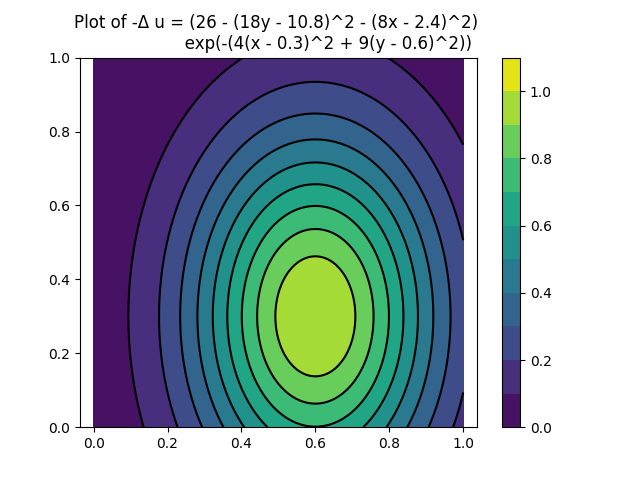
\includegraphics[width=.5\linewidth]{./test_plot_poisson.png}
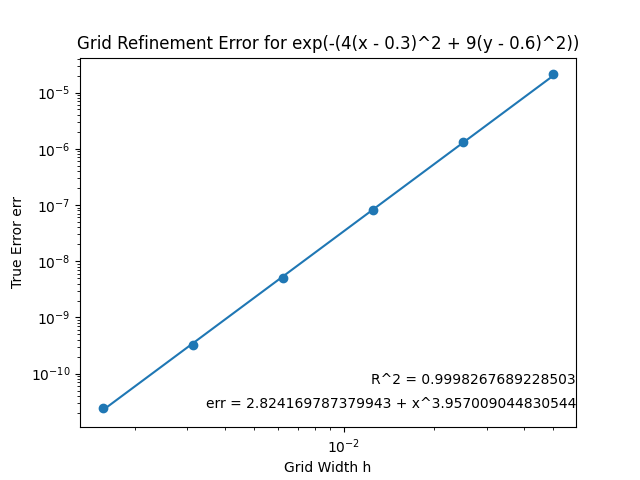
\includegraphics[width=.5\linewidth]{./error_plot_poisson.png}

\begin{verbatim}
"""
    Computes the discretization Au = b of -Δu = f on the unit square with boundary 
    condition u = g to 4th order in h = 1/n (the grid width)
    Optionally setting useadhoclaplace = false, giving the true laplacian Lap_f of f 
    uses that instead of using a 5 point scheme to estimate it.

    We achieve 4th order by using the 9 point Laplacian with error
    -Δ_9 u = -Δu - h^2/12 Δ^2 u + O(h^4)
    Since -Δu = f (for the true solution) we see that the scheme 
    -Δ_9 u = f + h^2/12 * Δf has order O(h^4), even if we use an order h^2 
    scheme to estimate Δf (which is done below)
"""
function assemblePoisson(n, f, g, useadhoclaplace =true, Lap_f = 0)
    h = 1.0/n
    N = (n+1)^2
    x = h* (0:n)
    y = x

    if useadhoclaplace
        Lap_f = adhocLaplace(f, h)
    else 
        Lap_f = (x,y) -> h^2 * Lap_f(x,y)
    end

    umap = reshape(1:N, n+1, n+1)
    A = Tuple{Int64, Int64, Float64}[]  #matrix of the finite difference as (row, col, val) 
                                        #row corresponds to output = forcing
                                        #col corresponds to input = u
    b = zeros(N)

    for j = 1:n+1
        for i = 1:n+1
            row = umap[i,j]
            if i == 1 || i == n+1 || j == 1 || j == n+1
                # On the boundary need to set u(x_i, y_j) = g(x_i, y_j)
                push!(A, (row, row, 1.0)) # 1 on the diagonal
                b[row] = g(x[i], y[j]) # value u should be 
            else 
                # In the interior use the 9 point stencil multiplied through by 6 h^2
                # Center
                push!(A, (row, row, 20.0))

                # Diagonals
                push!(A, (row, umap[i-1,j-1], -1.0))
                push!(A, (row, umap[i+1,j-1], -1.0))
                push!(A, (row, umap[i-1,j+1], -1.0))
                push!(A, (row, umap[i+1,j+1], -1.0))

                # Edges
                push!(A, (row, umap[i-1,j], -4.0))
                push!(A, (row, umap[i+1,j], -4.0))
                push!(A, (row, umap[i,j-1], -4.0))
                push!(A, (row, umap[i,j+1], -4.0))

                # Forcing
                # Note that we already multiplied by h^2 so 
                # really the laplace f term has h^4
                b[row] = 6 * h^2 * f(x[i], y[j]) + h^2/2.0 * Lap_f(x[i],y[j])
            end
        end
    end

    A = sparse((x->x[1]).(A), (x->x[2]).(A), (x->x[3]).(A), N, N)

    return A, b, x, y
end

"""
    Computes the 5 point Laplacian of a function f with grid size h, to avoid loss of 
    precision we avoid dividing by h^2
"""
function adhocLaplace(f, h)
    # for h sufficiently small we are losing some precision here by 
    # dividing by h^2 when # we're gonna multiply it by h^2 later 
    # anyway so we simply don't
    return (x,y) -> -4.0 * f(x,y) + f(x-h,y) + f(x+h, y) + f(x, y-h) + f(x,y+h)
end
\end{verbatim}


\newpage 

\problemitem[2a)] Introduce a mapping $T$ to transform the original domain $\Omega$ (with 
coordinates $x,y$) to the unit square $\hat \Omega$ (with coordinates $\xi, \eta$). Derive the 
equations and the boundary conditions in the new domain.
\prob

We will use the mapping 
$$T(x,y) = (\xi(x,y), \eta(x,y)) = 
\left(\frac{x}{B/2 + A/H y} , y/H\right)$$

To derive the equations we note that 
$$\pdiff x = \pdiff[\xi]x \pdiff \xi + \pdiff[\eta]x \pdiff \eta 
= \frac{1}{B/2 + A/Hy} \pdiff \xi$$
$$\pdiff y = \pdiff[\xi]y \pdiff \xi + \pdiff[\eta]y \pdiff \eta
= -\frac AH\frac{x}{(B/2 + A/Hy)^2} \pdiff \xi + \frac1H \pdiff \eta$$
It will be helpfull to have these entirely in terms of the unit square:
$$\pdiff x 
= \frac{1}{B/2 + A \eta} \pdiff \xi$$
$$\pdiff y 
= -\frac AH\frac{\xi}{B/2 + A\eta} \pdiff \xi + \frac1H \pdiff \eta$$
And in matrix form (in the standard basis $a\pdiff x + b \pdiff y$ is equal to)
$$
dT \begin{bmatrix} a \\ b\end{bmatrix} = 
\begin{bmatrix}
    \frac{1}{B/2 + A \eta} & -\frac AH\frac{\xi}{B/2 + A\eta}\\ 
    0 & \frac1H
    \end{bmatrix}
    \begin{bmatrix} a \\ b\end{bmatrix}$$


To calculate the Laplacian in $\hat \Omega$, we will need to make sense of second partials:
\begin{align*}
    -\left(\pdiff x\right)^2 &= -\left(\frac{1}{B/2 + A\eta} \pdiff \xi\right)\left(\frac{1}{B/2 + A\eta} \pdiff \xi\right)\\
    &= -\frac{1}{(B/2 + A\eta)^2} \left(\pdiff \xi\right)^2
\end{align*}
\begin{align*}
    -\left(\pdiff y\right)^2 
    &= -\left(-\frac AH\frac{\xi}{B/2 + A\eta}\pdiff\xi + \frac1H \pdiff\eta\right)
    \left(-\frac AH\frac{\xi}{B/2 + A\eta}\pdiff\xi + \frac1H \pdiff\eta\right)\\
    &= -\left(\frac AH\frac{\xi}{B/2 + A\eta}\right)^2\left(\pdiff \xi\right)^2
    +2 \frac A{H^2}\frac{\xi}{B/2 + A\eta} \pdiff \xi \pdiff \eta - \frac1{H^2} 
    \left(\pdiff \eta\right)^2\\
    &-\xi\left(\frac AH\frac{1}{B/2 + A\eta}\right)^2\pdiff \xi 
    - \left(\frac {A^2}{H^2}\frac{\xi}{(B/2 + A\eta)^2}\right) \pdiff \xi
\end{align*}

It follows that the Laplacian in the square is the sum of these.

For computing the flowrate it will be useful to have an expression for $dx \wedge dy$ 
in the new coordinates. For this we use the determinant
$$d\xi \wedge d\eta = \det dT dx \wedge dy = \frac1H \frac1{B/2 + A\eta} dx \wedge dy$$
So that 
$$\int_\Omega u(x,y) dx dy = \int_{\hat \Omega} u(\xi, \eta) H(B/2 + A \eta) d\xi d\eta$$

\newpage

\problemitem[2b)] In the transformed domain, write down second-order accurate finite-difference 
schemes for the discretization of all the derivative terms in the interior with Neumann boundary
conditions on the top and left (use the left condition for the upper left corner) and 
Dirichlet for the other two (use these for the remaining corners). Also show how to evaluate
the integral in the approximate flowrate $\hat Q$ numerically in the computational domain.
\prob

In the interior we approximate the usual way:
$$\p_\xi u(\xi, \eta) = \frac{1}{2h} \big(u(\xi + h, \eta)
- u(\xi - h, \eta)\big) + \O(h^2)$$
$$\p_\xi^2 u(\xi, \eta) = \frac{1}{h^2} \big(u(\xi + h, \eta) -2 u(\xi, \eta) 
+ u(\xi - h, \eta)\big) + \O(h^2)$$
$$\p_\xi\p_\eta u(\xi, \eta) = \frac{1}{4h^2} \big(u(\xi+h, \eta + h) -u(\xi-h, \eta+h) 
- u(\xi + h, \eta - h) + u(\xi - h, \eta - h)\big) + \O(h^2)$$
And similarly for $\eta$. Below we use the 
notation $\xi_i = h(i-1)$, $\eta_j = h(j-1)$, (I'm going to catch the indexing by 
1 issue here) and $u_{ij} = u(\xi_i, \eta_j)$.
Then, carefully counting we have that, $-\nabla^2$ in the 
computational coordinates becomes
\begin{align*}
1 = D u_{ij} &= \frac2{h^2}\left(\frac1{(B/2 + A\eta_j)^2} 
    + \left(\frac{A\xi_i}{H(B/2 + A\eta_j)}\right)^2 +  \frac1{H^2}\right) u_{ij}\\
             &+\frac1{4h^2}2\frac{A}{H^2}\frac{\xi_i}{B/2 + A\eta_j} 
             \left(u_{(i+1)(j+1)} - u_{(i+1)(j-1)} - u_{(i-1)(j+1)} + u_{(i-1)(j-1)}\right)\\
             &+\left(\frac{-1}{h^2}\frac{1}{(B/2 + A\eta_j)^2} 
         + \frac{-1}{h^2} \left(\frac{A}{H} \frac{\xi_i}{B/2 + A\eta_j} \right)^2
     +\frac{-1}{2h}2\xi_i\left(\frac AH\frac 1{B/2 + A\eta_j} \right)^2
 \right)u_{(i+1)j}\\
             &+\left(\frac{-1}{h^2}\frac{1}{(B/2 + A\eta_j)^2} 
         + \frac{-1}{h^2} \left(\frac{A}{H} \frac{\xi_i}{B/2 + A\eta_j} \right)^2
     +\frac{1}{2h}2\xi_i\left(\frac AH\frac 1{B/2 + A\eta_j} \right)^2
 \right)u_{(i-1)j}\\
             &+\frac{-1}{h^2}\frac 1{H^2} \big(u_{i(j+1)} + u_{i(j-1)}\big)
\end{align*}
Simplifying this some gives 
\begin{align*}
1 = D u_{ij} &= \frac2{h^2}\left(\frac{1+ A^2/H^2 \xi_i^2}{(B/2 + A\eta_j)^2} 
+ \frac1{H^2}\right) u_{ij}\\
             &+\frac1{2h^2}\frac{A}{H^2}\frac{\xi_i}{B/2 + A\eta_j} 
             \left(u_{(i+1)(j+1)} - u_{(i+1)(j-1)} - u_{(i-1)(j+1)} + u_{(i-1)(j-1)}\right)\\
             &+\left(\frac{-1}{h^2}\frac{1+A^2/H^2 \xi_i^2}{(B/2 + A\eta_j)^2} 
             +\frac{-1}{h}\frac {A^2/H^2\xi_i}{(B/2 + A\eta_j)^2}
 \right)u_{(i+1)j}\\
             &+\left(\frac{-1}{h^2}\frac{1+A^2/H^2 \xi_i^2}{(B/2 + A\eta_j)^2} 
             +\frac{1}{h}\frac {A^2/H^2\xi_i}{(B/2 + A\eta_j)^2}
 \right)u_{(i-1)j}\\
             &+\frac{-1}{h^2}\frac 1{H^2} \big(u_{i(j+1)} + u_{i(j-1)}\big)
\end{align*}

For the left boundary condition (excluding the bottom left corner) 
we use a right sided derivative. Note that 
$\p_\xi u = 0$ is equivalent to $\p_x u = 0$ so we don't need to compute the coefficient.
$$0 = \frac1{2h} (-3 u_{ij} + 4 u_{(i+1)j} - 1u_{(i+2)j})$$
For the top boundary (excluding the corner points) we use a centered derivative for 
$\p_\xi$ and a left sided derivative for $\p_\eta$
$$0 = -\frac{A/H \xi_i}{B/2 + A\eta_j} \frac1{2h}(u_{(i+1)j} - u_{(i-1)j})
+\frac1H \frac1{2h}(3u_{ij} - 4u_{i(j-1)} + 1u_{i(j-2)})$$

To calculate the flowrate we simply use the trapezoidal sum on 
$f(\xi, \eta) = H(B/2 + A\eta)u(\xi, \eta)$
which will work out to be 
$$\frac{h^2}{4} \left(f(0,0) + \cdots + f(1,1) +
2 \sum f(\xi_i, 0) + \cdots + 2 \sum f(1, \eta_j) 
+ 4 \sum f(\xi_i, \eta_j)\right)$$

\newpage

\problemitem[2c)] Make convergence plots and calculate convergence rates for the error in the output
$Q$.
\prob

Here are the plots, with linear regressions:

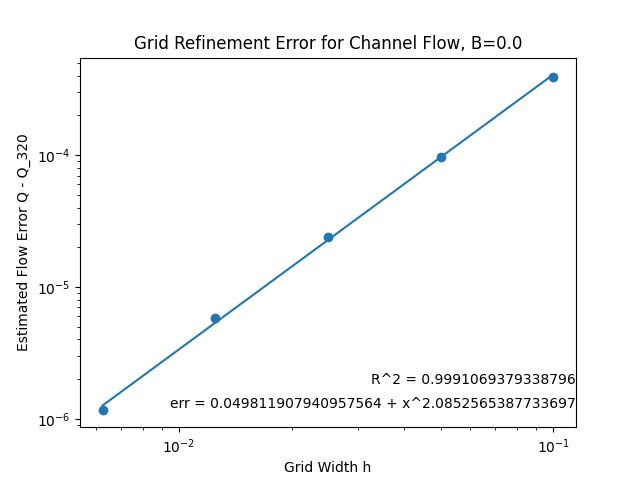
\includegraphics[width=.5\linewidth]{./error_plot_flow_0.0.png}
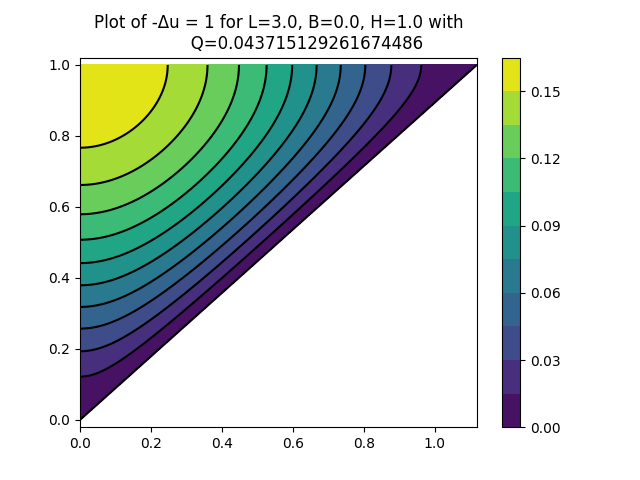
\includegraphics[width=.5\linewidth]{./test_plot_channel_0.0.png}

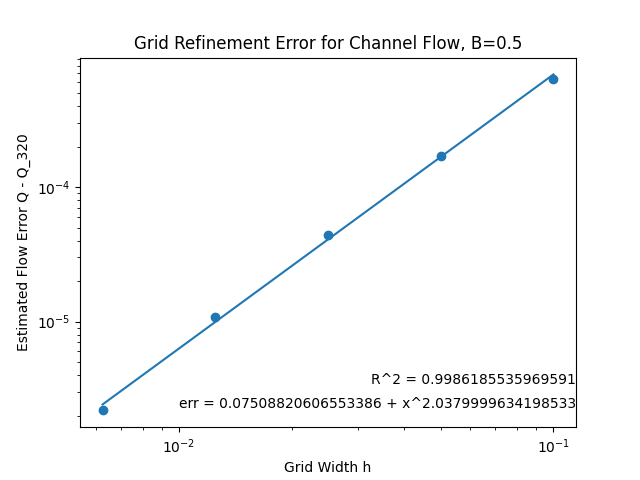
\includegraphics[width=.5\linewidth]{./error_plot_flow_0.5.png}
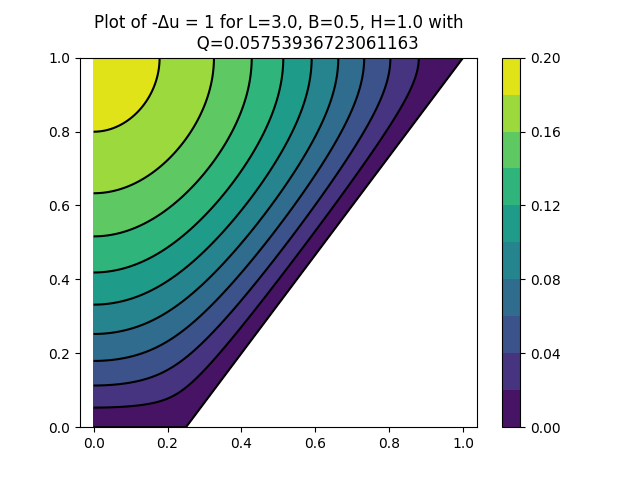
\includegraphics[width=.5\linewidth]{./test_plot_channel_0.5.png}

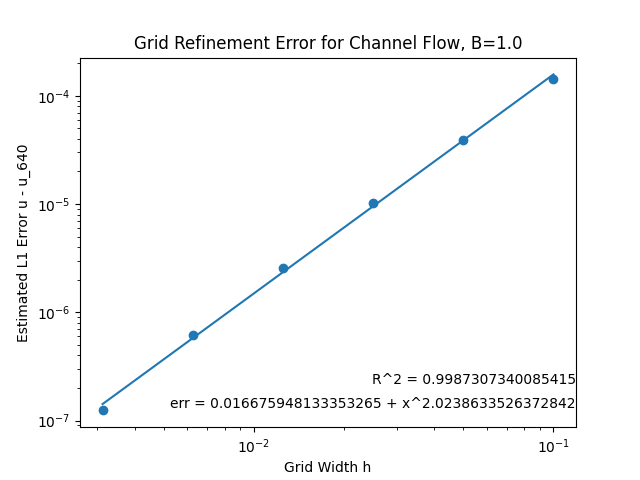
\includegraphics[width=.5\linewidth]{./error_plot_flow_1.0.png}
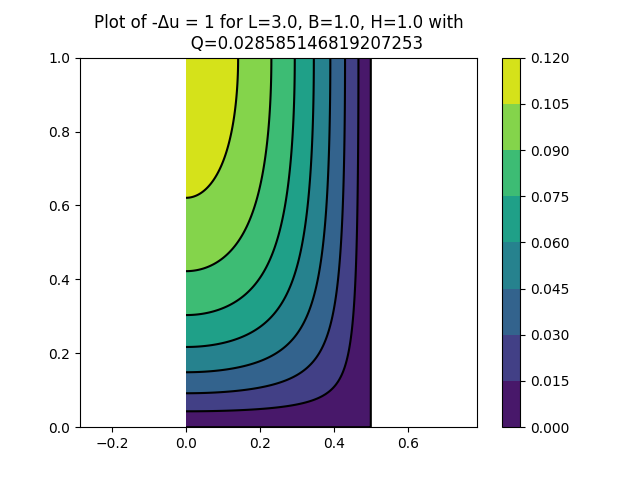
\includegraphics[width=.5\linewidth]{./test_plot_channel_1.0.png}

And the code 

\begin{verbatim}
function channelflow(L,B,H,n)
    h = 1.0/n
    N = (n+1)^2
    xi = h * (0:n)
    eta = xi
    A = sqrt((L - B)^2/4.0 - H^2)

    umap = reshape(1:N, n+1, n+1)
    M = Tuple{Int64, Int64, Float64}[]  #matrix of the finite difference as (row, col, val)
                                        #row corresponds to output = forcing
                                        #col corresponds to input = u
    b = zeros(N)
    for j = 1:n+1
        for i = 1:n+1
            row = umap[i,j]
            denom = 1.0/(B/2.0 + A*eta[j])
            if i == n+1 || j == 1
                # Dirichlet boundary
                push!(M, (row, row, 1.0)) # 1 on the diagonal
                b[row] = 0.0 # value u should be
            elseif i == 1
                # left boundary (before the upper boundary so the corner will live here)
                push!(M, (row, umap[i,j], -3.0))
                push!(M, (row, umap[i+1,j], 4.0))
                push!(M, (row, umap[i+2,j], -1.0))
                b[row] = 0.0 #multiply through by 2h
            elseif j == n+1
                # upper boundary (multiply through by 2hH)
                # xi part
                push!(M, (row, umap[i+1,j], -A*xi[i]*denom))
                push!(M, (row, umap[i-1,j], A*xi[i]*denom))
                # eta part
                push!(M, (row, umap[i,j], 3.0))
                push!(M, (row, umap[i,j-1], -4.0))
                push!(M, (row, umap[i,j-2], 1.0))
                b[row] = 0.0
            else
                # In the interior use the crazy mess we calculated
                # Being a bit more verbose to try to midigate errors
                # Center - contributions from 2nd derivatives
                push!(M, (row, umap[i,j], 2.0/h^2 *((1+A^2/H^2 *xi[i]^2)*denom^2 + 1/H^2)))

                # Diagonals - contributions from mixed derivatives
                push!(M, (row, umap[i+1,j+1], 1.0/h^2/2.0 *A/H^2 *xi[i]*denom))
                push!(M, (row, umap[i+1,j-1], -1.0/h^2/2.0 *A/H^2 *xi[i]*denom))
                push!(M, (row, umap[i-1,j+1], -1.0/h^2/2.0 *A/H^2 *xi[i]*denom))
                push!(M, (row, umap[i-1,j-1], 1.0/h^2/2.0 *A/H^2 *xi[i]*denom))

                # Horizontal edges - xi derivatives
                push!(M, (row, umap[i+1,j], -1.0/h^2*(1.0 + A^2/H^2 * xi[i]^2) * denom^2
                          - 1.0/h *A^2/H^2 * xi[i] * denom^2))
                push!(M, (row, umap[i-1,j], -1.0/h^2*(1.0 + A^2/H^2 * xi[i]^2) * denom^2
                          + 1.0/h *A^2/H^2 * xi[i] * denom^2))

                # Vertical edges - eta derivatives
                push!(M, (row, umap[i,j+1], -1.0/h^2/H^2))
                push!(M, (row, umap[i,j-1], -1.0/h^2/H^2))

                # Forcing
                b[row] = 1.0
            end
        end
    end

    M = sparse((x->x[1]).(M), (x->x[2]).(M), (x->x[3]).(M), N, N)

    # The solution reshaped into a square matrix (note we don't change anything here
    # because functions don't transform under change of variables - we just reinterpret the
    # grid)
    u = reshape(M \ b, length(xi), length(eta))
    # To get the original coordinates we use the inverse map - note that we can't have
    # x and y independent - we need them to be matrices of the same size as u
    x = [[i*(B/2.0 + A*j) for j in eta] for i in xi]
    y = [[H*j for j in eta] for i in xi]

    f(i,j) = H*(B/2 + A*eta[j])*u[i,j]

    Q = h^2/4.0 * (f(1,1) + f(1,n+1) + f(n+1,1) + f(n+1,n+1)
                   + 2*sum(f(i,1) for i in (2:n)) + 2*sum(f(i,n+1) for i in (2:n))
                   + 2*sum(f(1,j) for j in (2:n)) + 2*sum(f(n+1,j) for j in (2:n))
                   + 4*sum(f(i,j) for i in (2:n) for j in (2:n)))

    return Q, x, y, u
end

\end{verbatim}

\newpage

\problemitem[3a)] Show that the method 
$$U^{n+1}_j = U_j^n + \frac{k\kappa}{2h^2}
[U^n_{j-1} - 2U^n_j + U^n_{j+1}
U^{n+1}_{j-1} - 2U^{n+1}_j + U^{n+1}_{j+1} ]
-k\gamma[(1-\theta) U^n_j + \theta U^{n+1}_j]$$
for the PDE 
$$u_t = \kappa u_{xx} - \gamma u$$
(with $\kappa, \gamma > 0$)
is $\O(k^p + h^2)$ accurate where $p=2$ if $\theta = 1/2$ and $p=1$ otherwise.
\prob

We compute the local truncation error by plugging in a true solution to the scheme 
and Taylor expanding. For the sake of clarity let's deal with one thing at a time:

\begin{align*}
    \frac{u(x, t+k) - u(x, t)}{k} = 
    u_t(x,t) + \frac12 k u_{tt}(x,t) + \O(k^2),
\end{align*}
\begin{align*}
    -&\frac{\kappa}{2h^2}
    [u(x + h, t) - 2 u(x,t) + u(x-h, t) + u(x + h, t+k) - 2 u(x,t+k) + u(x-h, t+k)]\\
     &=-\frac\kappa2 u_{xx}(x,t) - \frac\kappa2 u_{xx}(x,t+k)+ \O(h^2)\\
     &=-\kappa u_{xx}(x,t) - \frac\kappa2 k u_{xxt}(x,t)+ \O(h^2 + k^2) 
\end{align*}
and 
$$\gamma[(1-\theta)u(x,t) + \theta u(x,t+k)] = 
\gamma[u(x,t) + \theta k u_t(x,t)] + \O(k^2)$$
Summing these gives the truncation error (I will drop the $(x,t)$ since we've written it 
all at one location)
\begin{align*}
\tau =    \left(u_t - \kappa u_{xx} + \gamma u\right)& 
+ \frac12 k \pdiff t\left(u_t - \kappa u_{xx} + 2\theta \gamma u\right) + \O(k^2 + h^2)\\
                                               & = 0 + \frac12 k (2\theta - 1) u_t + \O(k^2 + h^2)
\end{align*}
Thus, since we expect $u_t$ to not be uniformly 0, we can see that the truncation error 
is order $k^2 + h^2$ if $\theta = 1/2$ and $k + h^2$ otherwise.


\end{problems}
\end{document}
% vim: set fdm=expr foldexpr=(getline(v\:lnum)=~'^\\s*\\\\item.*'?'a1'\:(getline(v\:lnum)=~'^\\s*\\\\begin.enumerate.*'?'a1'\:(getline(v\:lnum)=~'^\\s*\\\\end.enumerate.*'?'s2'\:(getline(v\:lnum+1)=~'^\\s*\\\\item.*'?'s1'\:(getline(v\:lnum)=~'^\\s*\\\\end.document.*'?0\:(getline(v\:lnum)=~'Begin\ My\ Stuff'?1\:(getline(v\:lnum)=~'End\ My\ Stuff'?'<1'\:'='))))))):
